\chapter{Muistinhallinta} \label{Toinen luku}

Ohjelman muistin rakenteen ymmärtäminen on erityisen tärkeää tehokkaan muistin käytön saavuttamiseksi. Seuraavassa luvussa tullaan esittelemään miten muistin allokointi ohjelmissa toimii
ja millaisista muistialueista ohjelman muisti koostuu. Huomioitavaa on, että seuraavaksi esiteltävä sovelluksen muistin rakenne, on tyypillisin malli kuvaamaan, miten tietokoneohjelman muisti koostuu. Ohjelman muistin rakenteeseen vaikuttaa mm. käytössä oleva suoritinarkkitehtuuri, ohjelmointikielen kääntäjä sekä kääntäjien tarjoamat muistin optimointityökalut.

\section{Ohjelman muisti}

Ohjelman suorituksen aikainen muisti jakautuu erilaisiin muistialueisin. Koodiosa sisältää varsinaisesti ajettavan ohjelman binäärin eli ohjelmatiedoston, jonka prosessori suorittaa. Lisäksi ohjelmalla on olemassa dataosa, joka koostuu alustetusta datasta ja alustamattomasta datasta. Alustetun datan alueeseen kuuluvat globaalit ja staattiset muuttujat sekä vakioarvoiset muuttujat, joille on alustettu jokin arvo. Alustamattomassa data-alueessa on kaikki alustamaton data eli muuttujat, jotka ovat esitelty (engl. \textit{declare}), mutta joille ei ole annettu mitään arvoa. Näiden muistialueiden data allokoidaan ajettavan ohjelman muistiin jo käännön aikana (engl. \textit{compile time}) eli ohjelmointikielen kääntäjän kääntäessä lähdekoodin. Ohjelmalla on lisäksi myös kaksi muuta muistialuetta, pino ja keko. Tyypillisesti pino sijaitsee ylhäällä ja keko alhaalla ohjelman virtuaalisessa muistiavaruudessa.\cite{mmic2010} Pinon datan allokointi tapahtuu jo käännön aikana, kun taas keon datan allokointi tapahtuu vasta ohjelman ajon aikana (engl. \textit{runtime})\cite{ddm2015book}. Pinon allokoinnin määrittely ei ole aivan yksikäsitteistä. Yleisesti lähteissä määritellään, että allokointi tapahtuu käännön aikana, mutta jotkin lähteet määrittelevät, että allokointi tapahtuu ajon aikana. Tämä johtuu pinon allokoinnin luonteesta, sillä vaikka pinon hallintaan liittyvät ohjeet syntyvät jo käännön aikana, varsinainen itse datan osoitteistus tapahtuu ajon aikana. Tarkemmin heti järjestelmän alustuksen yhteydessä.

\begin{figure}[tbh]
{\begin{centering}
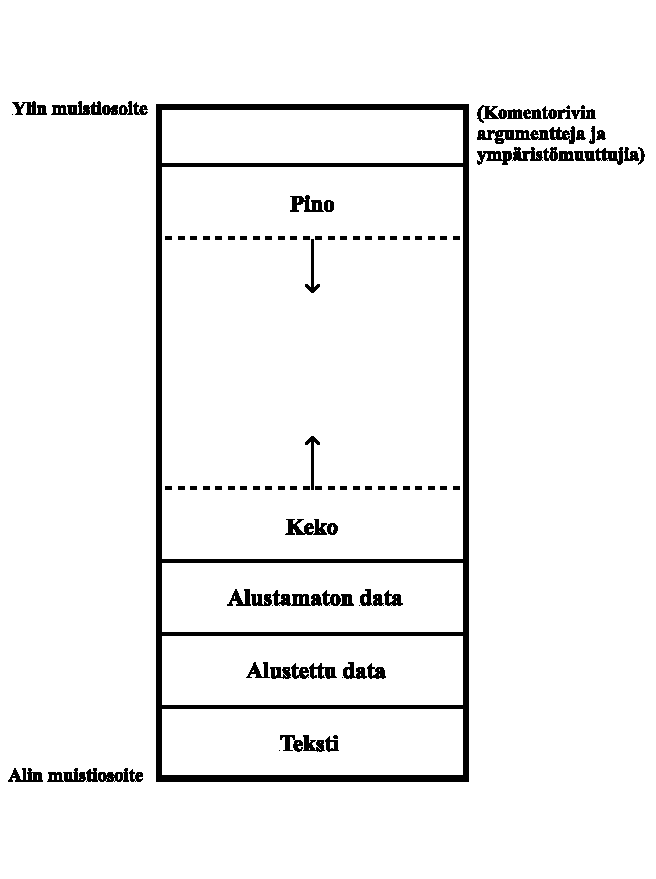
\includegraphics[width=0.6\textwidth]{kuvat/muistin_rakenne.pdf}
\par\end{centering}}
\caption{Ohjelman muistin rakenne \cite{mmic2010} (suomennettu kuva lähteestä)}
\end{figure}

\subsection{Pino}

Pino (engl. \textit{stack}) on ohjelman muistialue, johon allokoidaan paikalliset muuttujat, funktioiden parametrit ja paluuosoitteet. Se noudattaa LIFO-periaateetta (engl. \textit{Last In First Out}) eli pinoon viimeiseksi puskettu data poistetaan pinosta myös ensimmäisenä. LIFO-periaatteen ansiosta pinoallokointi on tyypillisesti nopeampaa kuin kekoon allokoiminen, johtuen tavasta, miten pinon dataan päästään käsiksi. Lisäksi, pinon tavuja käytetään ohjelmassa säännöllisesti yhä uudelleen ja uudelleen, jolloin ne säilyvät hyvin prosessorin nopeassa välimuistissa. Data allokoidaan pinoon automaattisesti ja poistetaan sieltä, kun sen näkyvyysalue päätyy. Pino koostuu kehyksistä (engl. \textit{frame}), joita pusketaan pinoon, kun ohjelma aloittaa uuden funktiokutsun suorittamisen. Tyypillisesti pinon koko on päätetty ennen ohjelman suorituksen aloittamista, ja pinoon allokoitavien muuttujien koko on tiedettävä etukäteen jo käännön aikana.\cite{mmic2010}
Pino-osoitin (engl. \textit{stack pointer}) pitää yllä tietoa muistiosoitteesta, jossa pinon viimeinen elementti sijaitsee. Tätä osoitinta muuttamalla, ohjelma pitää yllä tietoa mihin uusi kehys lisätään tai mistä vanha kehys poistetaan. Pino-osoittimen arvo pienenee, kun dataa pusketaan pinoon ja vastaisuudessa kasvaa, kun dataa poistetaan pinosta (huomioi pinon sijainti ohjelman muistiavaruudessa, kts. kuva 2.1).\cite{sasp2006}

\subsection{Keko}

Keko (engl. \textit{heap}, suom. myös \textit{kasa}) on muistialue, johon kehittäjä allokoi sekä josta myös vapauttaa muuttujat manuaalisesti. Keko sisältää käytettävissä olevien ja vapaiden muistilohkojen linkitetyn listan. Keolle annetaan aloituskoko ohjelman suorituksen alkaessa, mutta muistinvaraaja voi pyytää sitä lisää tarvittaessa käyttöjärjestelmältä. Vastapainona pinolle, keko on hyödyllinen, kun ei voida tietää etukäteen kuinka paljon muistia tarvitsee varata ajon aikana.\cite{mmic2010} On syytä mainita, että tietokoneohjelman muistialue keko ei ole sama asia kuin tietorakenne keko.

Ohjelmalistaus 1 on käytännön esimerkki, joka havainnollistaa mihin muistialueeseen kukin koodirivi sijoittuu ohjelman muistissa.

\begin{algorithm}[tbh]
\begin{lstlisting}[language=C]
#include <stdio.h>
#include <stdlib.h>

//Alustamaton muuttuja --> alustamaton data
int i;
//Alustettu muuttuja --> alustettu data 
int n = 1; 

//Funktiokutsu --> Pino
int main(void)  
{  
    //Paikallinen muuttuja --> Pino
    int numero = 10;
    //Dynaamisesti allokoitu muistilohko --> Keko    
    int* osoitin = (int*)malloc(n * sizeof(int));
    //Dynaamisesti vapautettu muistilohko --> Vapautettu keosta  
    free(osoitin);
    return 0;
}
\end{lstlisting}
\caption{Demonstraatio muistin allokoinnista C-ohjelmointikielessä\label{alg:Demonstraatio}}
\end{algorithm}

\section{Muistin allokointi ohjelmointikielissä}

Tietokoneohjelmissa hyödynnettävät muistinallokointimenetelmät jaotellaan tyypillisesti staattiseen allokointiin ja dynaamiseen allokointiin. Staattinen allokointi tarkoittaa muistilohkojen allokointia niin, että lohkot allokoidaan sovellukselle välittömästi järjestelmän alustuksen jälkeen. Näillä lohkoilla on ennaltamääritetty koko, joka määritetään käännön aikana. Tämän jälkeen järjestelmä ei allokoi enää lisää muistia, jollei kehittäjä sitä itse allokoi lisää dynaamisesti, vaan kaikki tehtävät ja prosessit suoritetaan näissä lohkoissa. Staattisen allokoinnin heikkous on muistilohkojen ennaltamäärätty koko. Allokoiduilla lohkoilla on kiinteä koko, jota ei pysty jälkikäteen muuttamaan. Tämä aiheuttaa haasteen, että kehittäjän on tiedettävä sopiva lohkon muistikoko etukäteen. Staattisen allokoinnin vastakohta on dynaaminen allokointi, missä muistilohkot allokoidaan globaalista muistiavaruudesta ohjelman ajonaikana tehtävän tai prosessin koon mukaan. Muistilohko vapautetaan, kun prosessi on valmis. Dynaamisen allokoinnin etuja ovat joustavuus ja muistinkäytön hyötysuhteen paraneminen, mutta dynaaminen allokointi heikentää järjestelmän vakautta.\cite{daroemmfera@2006}Muistinkäytön hyötysuhteen paranemisella tarkoitetaan, että dynaamisella allokoinnilla muistia voidaan käyttää vain juuri sen verran kuin on pakko. Staattisessa allokoinnissa muistia joudutaan monesti varaamaan hieman ylimääräistä, koska kokoa ei pystytä jälkikäteen muuttamaan. Tämä aiheuttaa sen, että ohjelman ajonaikana staattisesti varattua muistia voi olla paljon käyttämättömänä, koska sitä on varattu varmuudenvuoksi hieman ylimääräistä.

Dynaamista muistinhallintaa varten ohjelmointikielet tarjoavat erilaisia valmiista kirjastoista saatavia funktioita muistin varausta ja vapauttamista varten. C-ohjelmointikielessä funktio, jolla varataan muistia on malloc(), joka ottaa vastaan argumenttina muistin koon tavuina. Muistia vapautetaan funktiolla free(), joka ottaa parametrina osoittimen osoittaman muistilohkon. Lisäksi, on olemassa calloc() ja realloc(), joilla voi myös varata muistia. Calloc() ottaa kaksi argumenttia, joista toinen on varatun muistilohkon koko ja toinen määrittää kuinka monta näitä lohkoja varataan. Malloc()- ja calloc()-funktioiden keskeinen ero on, että calloc()-funktio myös alustaa varatun muistialueen nolliksi. Malloc() ei tätä alustusta suorita, vaan malloc()-funktion varaama muistialue sisältää mielivaltaisia alustamattomia arvoja.\cite{c2015book}Nämä mielivaltaiset alustamattomat arvot ovat siis joitain satunnaisia arvoja, jotka ovat jääneet muistiosoitteeseen edellisestä muistin varauksesta. Realloc() on funktio, jolla pystyy muokkaamaan jo aikaisemmin varatun muistialueen kokoa. Realloc() ottaa argumentikseen muokattavan muistialueen osoittimen sekä muistilohkon uudelleen määritetyn koon\cite{c2015book}.

\section{Muistinhallinnan ongelmatilanteet}

\begin{figure}[tbh]
{\begin{centering}
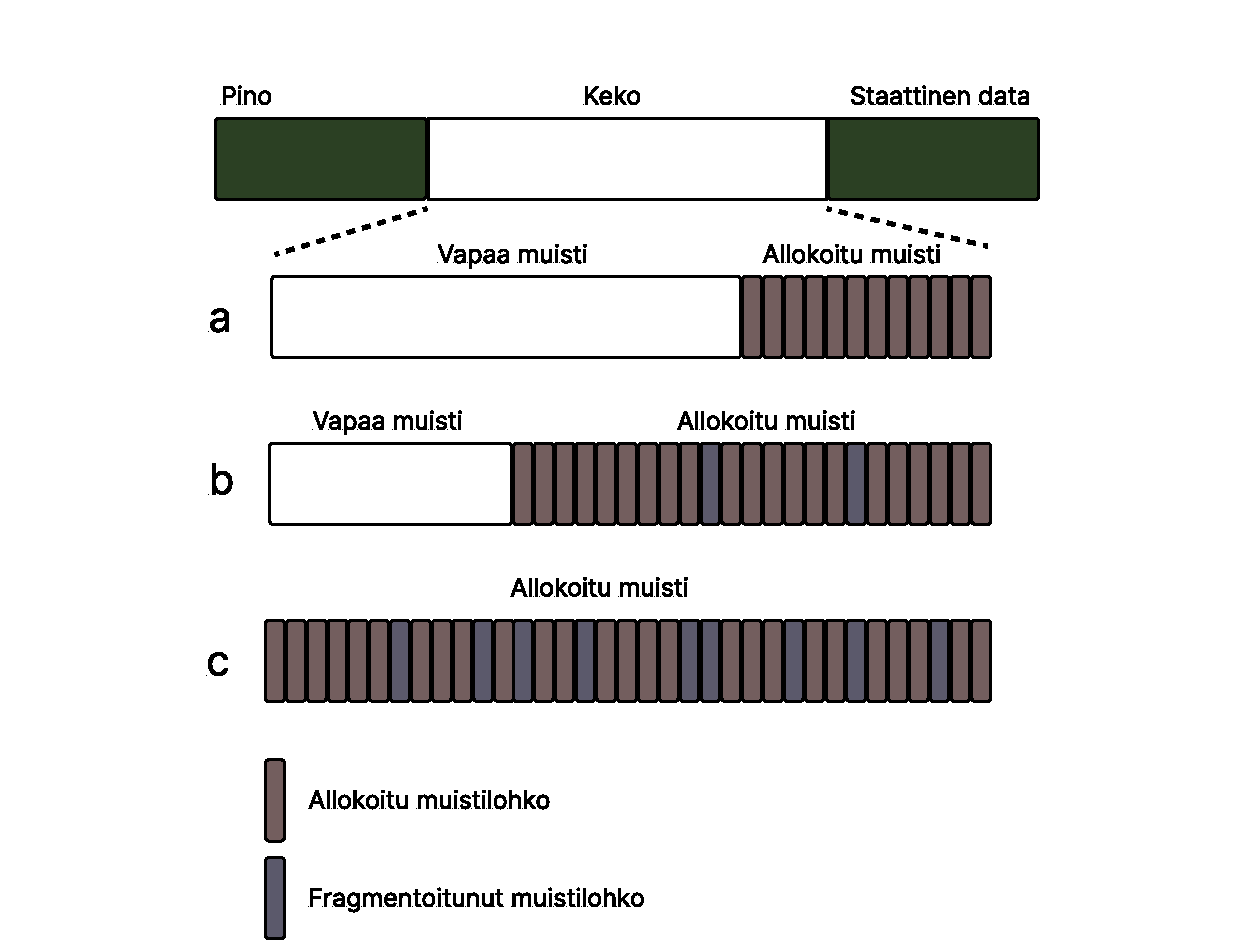
\includegraphics[width=0.8\textwidth]{kuvat/fragmentaatio.pdf}
\par\end{centering}}
\caption{Muistin fragmentoituminen\cite{ammsfmes@2016}(suomennettu kuva lähteestä)}
\end{figure}

Muistin fragmentoituminen on muistin tila, jossa usein tapahtuva muistilohkojen allokointi ja vapautus on aiheuttanut sen, että ohjelma ei kykene enää varaamaan käyttöönsä riittävän suurta jatkuvaa muistilohkoa, vaan vapaa muisti on pirstoutunut yksittäisiksi lohkoiksi jo allokoitujen lohkojen välin. Muistin fragmentoitumista pidetään yhtenä sulautettujen järjestelmien muistinkäytön haasteena.\cite{ammsfmes@2016}Kuva 2.2 havainnollistaa muistin fragmentoitumisen erilaisia tiloja. A-kuva on ideaalitilanne, jossa muisti ei ole olleenkaan fragmentoitunut. B-kuvassa kaksi lohkoa on jäänyt allokoitujen lohkojen väliin. C-kuvassa muisti on jo pahasti fragmentoitunut. Fragmentoituneet lohkot ovat vapaita lohkoja, mutta koska ne eivät muodosta ohjelman muistiavaruudessa jatkuvaa tyhjää tilaa, yksittäisiä vapaita lohkoja suuremmat tietorakenteet eivät pysty tätä tyhjää muistitilaa hyödyntämään.

Muistivuoto on muistinkäytön ongelmatilanne, joka tapahtuu kun ohjelma käyttää muistia, mutta ei kykene vapauttamaan sitä takaisin käyttöjärjestelmän käyttöön. Muistivuodot ovat hyvin ikäviä ongelmatilanteita, sillä niiden jäljittäminen vaatii pääsyn ohjelman lähdekoodiin, ja monesti muistivuodot ilmenevät ohjelmassa lukuisina muina ongelmina. Usein ajatellaan virheellisesti, että yleisesti ohjelman lisääntynyt muistinkäyttö on muistivuoto, vaikka tämä ei pidä paikkaansa. Monesti muistivuodot eivät ilmene ohjelmaa ajettaessa välittömästi, vaan hitaasti ohjelman ajon aikana, kun ohjelma varaa yhä enemmän ja enemmän muistia. Lopulta tämä ilmenee ohjelman kaatumisena tai käyttöjärjestelmän hidastumisena.\cite{mmic2010}

Dynaaminen muistinhallinta tuo kehittäjälle vapautta, mutta myös suuren vastuun. Aikaisemmin mainitut muistinkäytön ongelmatilanteet ja virheet voivat aiheuttaa päänvaivaa kokemattomalle kehittäjälle, mutta kokeneelle kehittäjälle osoittimet ja manuaalinen allokointi tarjoavat tehokkaat työkalut sovelluksen muistinkäytön tehostamiselle. Ohjelmointikielissä, jotka tarjovat kehittäjälle dynaamisen muistinhallinnan mahdollisuuden, kehittäjän on hyvin tärkeää ymmärtää, miten ohjelman muisti toimii, jotta näiltä onglematilanteilta vältytään.


